\chapter{Validation of \pharmml}
\label{chapter:validation}

\newenvironment{valrules}{\begin{description}}{\end{description}}
\newcommand*{\valrule}[2]{\item[#1] \emph{#2}}

% Redefine row gaps for these tables.
\renewcommand{\arraystretch}{1.25}


\section{Introduction}

In this section we provide detailed rules about what constitutes a
valid \pharmml document. Where possible we have tried to keep each
rule definition discrete and also we have provided a unique
identifier for such rules. We recommend that developers implementing
support for \pharmml validation report such rule identifiers in their
error messages. Users can then cross-reference such errors with this
specification if they require more detailed information.

The rules are organised so that we cover the basic language features
and constructs first and then go into specific rules for each of the
sections of a \pharmml document: Model Definition, Trial Design and
Modelling Steps.

\section{Namespaces and Scopes}
\label{sec:symbolScoping}

\subsection{Defining Symbols and Objects}

\begin{figure}
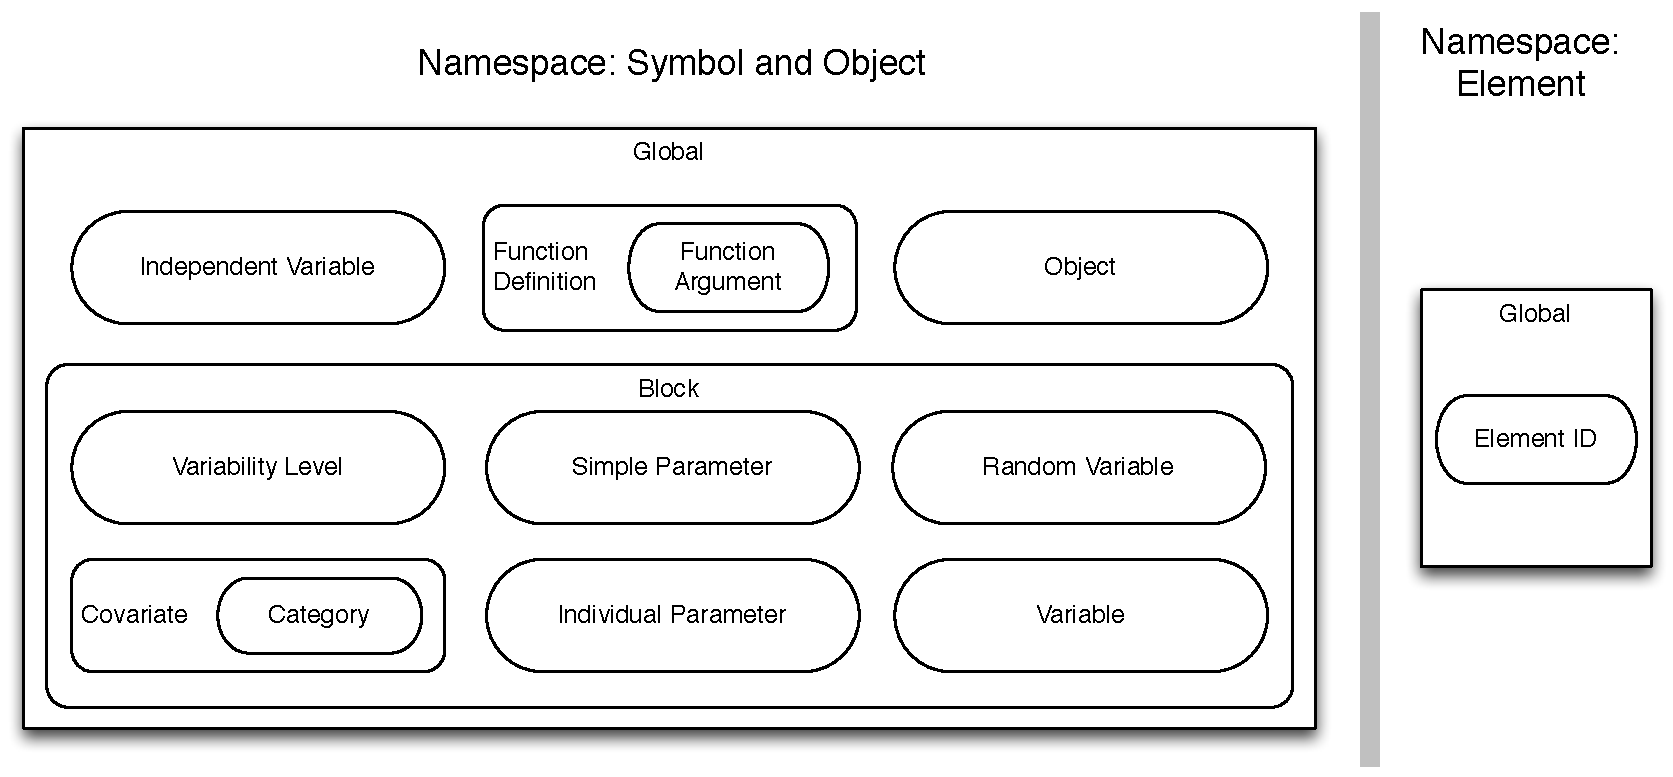
\includegraphics[width=\linewidth]{figures/scope_namespaces_overview}
\caption{An overview of the scopes and namespaces used in
  \pharmml. The class of symbols within the scope are shown as
  ovals, symbols that also define a scope are rounded rectangles
  and the global scope is shown as rectangles. So for example, the
  function argument is a class of symbol that is scoped by the
  function definition which in turn belongs to the global scope.}
\label{fig:scopes-overview}
\end{figure}

The namespaces and scopes used in \pharmml are shown in
figure~\ref{fig:scopes-overview}. By namespace we mean a
dictionary of names, in which each name must be unique within its
given scope. As you can see from the figure there are
two namespaces, one which defines the symbols used to describe the
model (for more background information read section~\ref{sec:blocks})
and the other (namespace Element) is used to allow the \pharmml
document to be cross references externally (see
section~\ref{sec:element-id}).  The symbols can be classified as
follows:
\begin{description}
\item[Independent Variable] A special variable that defines the
  independent variable used throughout the model.
\item[Function Definition] A function that can be reused throughout
  the \pharmml document.
\item[Function Argument] The parameters of the function. Their scope
  extends into the body of the function. For example: $f(x) = x + 1$.
\item[Object] An identifier used to uniquely identify conceptual
  objects within the \pharmml document.
\item[Block] An identifier that defines a model within the Model
  Definition section of \pharmml. This provides a scope for symbols
  defined within the block and gives the model definition a degree of
  modularity.
\item[Variability Level] A symbol that defines a level of random
  variability.
\item[Covariate] A symbol that defines variability associated with an
  individual. It can be continuous or categorical. In the latter case
  categories are scoped by the covariate symbol.
\item[Category] A category of a categorical covariate.
\item[Simple Parameter] A parameter that cannot be assigned a random variable.
\item[Individual Parameter] A parameter that can be assigned a random
  variable.
\item[Random Variable] A special parameter than is described by a
  probability distribution.
\item[Variable] A variable in the model. This is distinguished from a
  parameter in that it can change over time, while a parameter cannot.
\item[Element ID] An identifier used by external resources to identify
  a specific element within the \pharmml document.
\end{description}
%
Using these concepts we can apply the following rule:
%
\begin{valrules}
  \valrule{S1}{Symbols must be unique with their scopes.} Duplicate
  symbols are not permitted within a given namespace.
\end{valrules}

\subsection{Symbol Resolution}
\label{sec:ref-symbol-resolution}

Symbols must be resolved using the scoping rules. This is described in
detail in section~\ref{sec:blocks}. Symbols are typically referred to
using the \xelem{SymbRef} element and objects by the \xelem{OidRef} element
or XML elements of type OidRefType. Resolution rules are:

\begin{valrules}
\valrule{S2}{References to symbols and objects must resolved.}
Dangling references are not permitted.
\valrule{S3}{The resolved symbol must be compatible with the \pharmml
  component referencing it.} This means that an \xelem{ArmRef}
which should match an arm definition should not point to an Epoch
definition. Compatibility is defined in the table \ref{tab:symbref-targets}.
\valrule{S4}{A \xelem{SymbRef} element must only reference symbols
  that are compatible with its parent element.} Compatibility is
defined by table~\ref{tab:symbref-targets}.  
\valrule{S5}{A \xelem{OidRef} element or element using the type
  \texttt{OidRefType} must only reference objects
  that are compatible with its parent element.} Compatibility is
defined by table~\ref{tab:oidref-targets}.  
\end{valrules}


%\begin{table}[ht!]
%\begin{center}
\begin{center}
\small
\begin{longtable}{ll}\toprule
Reference Parent & Target \\\midrule
VariableAssignment & SimpleParameter, CovariateModel/Covariate, RandomVariable \\
 & IndividualParameter, Variable, DerivativeVariable \\
ParentLevel & VariabilityModel/Level (The correct target is
  also affected by rule M6.) \\
PopulationParameter & SimpleParameter \\
LinearCovariate/Covariate & CovariateModel/Covariate \\
FixedEffect & SimpleParameter \\
GeneralCovariate & SimpleParameter, CovariateModel/Covariate \\
GaussianModel/\-RandomEffects & RandomVariable \\
IndividualParameter/\-Assign &  SimpleParameter,
CovariateModel/\-Covariate, RandomVariable, \\ 
& IndividualParameter \\
VariabilityReference & VariabilityModel/Level \\
SimpleParameter & SimpleParameter \\
RandomVariable1 & RandomVariable \\
RandomVariable2 & RandomVariable \\
CorrelationCoefficient & SimpleParameter \\
Covariance & SimpleParameter \\
Variable & SimpleParameter, CovariateModel/Covariate, RandomVariable, \\ 
& IndividualParameter, Variable, DerivativeVariable \\
DerivativeVariable/Assign & SimpleParameter, CovariateModel/Covariate, RandomVariable, \\ 
& IndividualParameter, Variable, DerivativeVariable \\
DerivativeVariable/\-IndependentVariable & Variable \\
InitialCondition & SimpleParameter, CovariateModel/Covariate, RandomVariable, \\ 
& IndividualParameter,Variable,DerivativeVariable \\
ObservationModel/\-General &  SimpleParameter,
CovariateModel/\-Covariate, RandomVariable, \\
& IndividualParameter \\
ObservationModel/\-Standard/\-Output & Variable, DerivativeVariable \\
ErrorModel &
FunctionDefinition, SimpleParameter, IndividualParameter, \\
& RandomVariable\\
RandomError & RandomVariable \\
DoseAmount & Variable, DerivativeVariable\footnote{The choice of
 valid target is governed by rules D11-13.}\\
SteadyState/EndTime & Variable, DerivativeVariable \\
SteadyState/Interval & Variable, DerivativeVariable \\
DosingTimes & Variable, DerivativeVariable \\
Duration & Variable, DerivativeVariable \\
Rate & Variable, DerivativeVariable \\
CovariateMapping & Covariate \\
SimulationStep/Observations/\-Continuous & Variable/DerivativeVariable
\\
ParameterEstimation & SimpleParameter, IndividualParameter, Covariate \\
InitialEstimate & Variable, DerivativeVariable, FunctionDefinition, SimpleParameter, \\
& IndividualParameter, RandomVariable \\
LowerBound & Variable, DerivativeVariable, FunctionDefinition, SimpleParameter, \\
& IndividualParameter, RandomVariable \\
UpperBound & Variable, DerivativeVariable, FunctionDefinition, SimpleParameter, \\ 
& IndividualParameter, RandomVariable \\\bottomrule
\caption{This table describes the compatibility of symbol
  references defined using \xelem{SymbRef}. The comparability is with
  the parent elements that use the \xelem{SymbRef} to refer to other
  symbols within the \pharmml document. In the table the Reference
  Parent column describes the element which is the immediate parent of
  the \xelem{SymbRef} element. The target column specifies the set
  of elements that can be the target of this reference. Where the
  parent element is required to identify the correct element a 'path'
  is indicated using the '/' symbol.}
\label{tab:symbref-targets}
%\end{table}%
\end{longtable}
\end{center}


\begin{table}[ht!]
\begin{center}
\small
\begin{tabular}{ll}\toprule
Reference Parent & Target \\\midrule
EpochRef & Epoch \\
ArmRef & Arm \\
SegmentRef & Segment\\
ActivityRef & Activity \\
DemographicMapping & Demographic\\
Step & SimulationStep, EstimationStep \\
Dependents & SimulationStep, EstimationStep \\\bottomrule
\end{tabular}
\end{center}
\caption{This table describes the compatibility of object
  references defined using \xelem{OidRef} or from elements of type
  \texttt{OidRefType}. The comparability is with the parent elements
  that use the above elements to refer to objects within the \pharmml
  document. In the table the Reference Parent column describes the
  element which is the immediate parent of the reference element. The
  target column specifies the set of elements that can be the target
  of the reference. Where the parent element is required to identify
  the correct element a 'path' is indicated using the '/'
  symbol.}
\label{tab:oidref-targets}
\end{table}%


\section{Type System}

\subsection{Types}

\pharmml has the types in the table \ref{tab:type-specification}. Some types can be
automatically converted (promoted) to another type. The rules are
described below, with detailed information provided in the specified tables.

\begin{valrules}
\valrule{S6}{\pharmml has a type system and all symbols and elements,
  if they have a type must conform to it.} The types are specified in table~\ref{tab:type-specification}.
\valrule{S7}{Symbol classes have a type.} The types are specified in table~\ref{tab:symbol-class-types}.
\valrule{S8}{Elements, that are explicitly typed must be associated with quantities of same type} Quantities
associated elements in a \pharmml document, must be of the same
type. The type of the relevant elements are described in
table~\ref{tab:element-types}.
\valrule{S9}{Literal values have a type.} The types of literal values
are specified in table~\ref{tab:literal-types}.
\end{valrules}

\begin{table}[ht!]
\begin{center}
\small
\begin{tabular}{lll}\toprule
Name & Promotion & Definition \\\midrule
real & real & Values of this type should conform to
  the double type defined by XML Schema \\
  & & (see \url{http://www.w3.org/TR/xmlschema-2/#double}).\\
  int & real & Values of this type should conform to
  the integer type defined by XML Schema \\
  & & (see \url{http://www.w3.org/TR/xmlschema-2/#integer}).\\
  array & array & A one-dimensional array of \texttt{real} values.\\
  string & string & The definition of string
  conforms to the XML Schema definition \\
  & & (see \url{http://www.w3.org/TR/xmlschema-2/#string}).\\
  boolean & boolean &  A two-valued logic value (True or False). In
  \moml we comply with the XML Schema \\
  & & definition (see \url{http://www.w3.org/TR/xmlschema-2/#boolean}). \\
  id & id & An identifier string, defined as equivalent to a non-colonised named in
  XMl Schema \\
  & & (see \url{http://www.w3.org/TR/xmlschema-2/#NCName}).\\
  void & void & A non-type. For consistency in defining language rules it is useful 
  to give some symbols \\
  & &  a type that do not have one in any meaningful sense. In such
cases we use this type. \\\bottomrule
\end{tabular}
\end{center}
\caption{Symbols can be created using these types. The types that can be used
with each symbol class can vary. In other cases the type is
implicit. This information is defined in the table below. Note that if
the type is ``explicit'' then this means that the range of possible
types are specified in the XML document and that the possible types are
encoded in the XML Schema definition.}
\label{tab:type-specification}
\end{table}%

%\begin{table}[ht!]
%\begin{center}
%\small
%\begin{tabular}{rrrrrrr}\toprule
%
%\end{tabular}
%\end{center}
%\caption{}
%\end{table}%


\begin{table}[ht!]
\begin{center}
\small
\begin{tabular}{ll}\toprule
 Symbol class & Type \\\midrule
 Independent Variable & real\\
Function Definition & string, real, boolean, id, int\\
Function Argument & string, real, boolean, id, int\\
Object & void\\
Block & void\\
Variability Level & void\\
\multirow{2}{*}{Covariate} & continuous: real \\
                & categorical: id \\
Simple Parameter & real \\
Individual Parameter & real \\
Random Variable & real \\
Variable & string, real, boolean, id, int\\
Element ID & void\\\bottomrule
\end{tabular}
\end{center}
\caption{Each symbol class has one or more types that it can be
  assigned to.}
\label{tab:symbol-class-types}
\end{table}%


\begin{table}[ht!]
\begin{center}
\small
\begin{tabular}{ll}\toprule
Element & Type \\\midrule
PopulationParameter & real \\
FixedEffect & real \\
GeneralCovariate & real \\
GaussianModel/\-RandomEffects & real \\
RandomVariable1 & real \\
RandomVariable2 & real \\
CorrelationCoefficient & real \\
Covariance & real \\
DerivativeVariable/\-IndependentVariable & real \\
InitialTime & real\\
InitialValue & real\\
ObservationModel/\-General &  real \\
ObservationModel/\-Standard/\-Output & real \\
ErrorModel & real \\
RandomError & real \\
DoseAmount & real \\
SteadyState/EndTime & real \\
SteadyState/Interval & real \\
DosingTimes & real \\
Duration & real \\
Rate & real \\
SimulationStep/Observations/\-Continuous & real\\
SimulationStep/Observations/\-Discrete & real\\
Property & real, int, string, boolean or array\\\bottomrule
\end{tabular}
\end{center}
\caption{As well as symbols defined by the language quantities can be
represented by constructs or concepts in the XML document. In many
cases such quantities are assigned by an \xelem{Assign} element. To
ensure type consistency we must understand the type of the quantity on
its left-hand side.}
\label{tab:element-types}
\end{table}%


\begin{table}[ht!]
\begin{center}
\small
\begin{tabular}{lll}\toprule
Literal & Type & Example \\\midrule
Real & real & \verb|<Real>22.3</Real>|\\
Int & integer & \verb|<Int>22</Int>|\\
String & string & \verb|<String>Hel lo</String>|\\
ID & id & \verb|<Id>hel10</Id>|\\
True & boolean & \verb|<True/>|\\
False & boolean & \verb|<False/>|\\\bottomrule
\end{tabular}
\end{center}
\caption{In common with other computational languages \pharmml provides a
mechanism to define literal values. In all cases these literals has a
type.}
\label{tab:literal-types}
\end{table}%


\section{Common Constructs}

\subsection{Assignment}
\label{subsec:AssinmentRules}

An assignment operation evaluates an expression, that may be a literal
value, a reference to a symbols or a mathematical equation. It then
associates that expression with a symbol, such as variable, parameter
or covariate, or with an element in the XML document. An assignment is
indicated by the \xelem{Assign} element. The following rules apply:

\begin{valrules}
  \valrule{S10} {No circular assignment for non-derivative symbols.} A
  circular assignment occurs if a symbol is initialised with an
  expression that when traced through the definition of each symbol in
  the expression ends back where it started. This generally
  prohibited, but permitted if the symbol being initialised is of
  derivative type. See section \ref{sec:blocks} for a more detailed
  description.
%
  \valrule{S11}{A symbol can be assigned only once.} See section
  \ref{sec:blocks}.
%
\valrule{S12}{Both sides of an assignment must have the same type.}
This means that the expression (the right-hand side of the assignment)
must evaluate to have a type that is identical to that of the symbol
or element it is to be associated with (the left-hand side).
\end{valrules}

\subsection{Mapping to a Dataset}

Elements map the symbol or model to a column in the \xelem{DataSet}
using the \xelem{ColumnRef} element. This gives us the following rules:

\begin{valrules}
  \valrule{S13}{A column reference must always resolve to a
    column in its associated dataset.} The associated dataset is clear
  from the content of reference in the XML Schema structure. To
  resolve correctly the value \xatt{columnIdRef} attribute must be identical
  to that of the \xatt{columnId} attribute in Column definition of
  dataset.
\valrule{S14}{A mapping between a symbol or object and a column in a
  dataset must be type consistent.} By this we mean that the type of
the object or element (defined in the table~\ref{tab:data-set-mapping}) must be the same as
the type specified in the column definition of the dataset.
\valrule{S15}{Mapping of derivative variables} If dosing target is 
\texttt{derivativeVariable} then the dosing variable must be a
derivative variable.
\valrule{S16}{Mapping of non-derivative variables} If dosing target is 
\texttt{variable} or \texttt{parameter} then the dosing variable must be a
non-derivative variable.
\valrule{S17}{Mapping of PK macros} If dosing target is \texttt{admType} 
then the dosing is aimed at a PK macro \emph{depot}, \emph{absorption}, 
\emph{oral} or \emph{iv}.
\valrule{S18}{Mapping of column with \xatt{columnType="id"}} Dataset column 
with \xatt{columnType="id"} must be mapped to the variability level representing
the subject if more then the reference level are defined in a variability model.
\valrule{S19}{Multiple DV mapping.} The use of \xelem{CategoryMapping} element
is allowed within \xelem{Piecewise} only in the context of multiple DV mapping
as implemented using \xelem{MultipleDVMapping}.
\end{valrules}

%\begin{table}[ht!]
%\begin{center}
%\small
%\begin{tabular}{rrrrrrr}\toprule
%
%\end{tabular}
%\end{center}
%\caption{}
%\end{table}%

\begin{table}[ht!]
\begin{center}
\small
\begin{tabular}{llll}\toprule
Mapping Element & Column Type & Value type & Target of Mapping \\\midrule
ColumnMapping & idv & real & IndependentVariable  \\
			& id			& id/string & VariabilityModel/Level \\
			& covariate & id/string &  ModelDefinition/Covariate (categorical) \\	
			& covariate & real &  ModelDefinition/Covariate (continues) \\
			& covariate & int &  ModelDefinition/VariabilityModel \\
			& dose 	& real &  ModelDefinition/DerivativeVariable, Variable \\
			& dv 	& real &  ModelDefinition/ObservationModel \\
DemographicMapping & & scalar & Demographic \\
IndividualDosing/DoseAmount & & real & DosingRegimen/*/DoseAmount \\
IndividualDosing/DosingTime & & real & DosingRegimen/*/DoseAmount \\
IndividualDosing/Rate &  & real & Infusion/Rate \\
IndividualDosing/Duration & & real &Infusion/Duration \\
IndividualDosing/SSEndTime & & real & SteadyState/EndTime \\
IndividualDosing/SSPeriod & & real & SteadyState/Interval \\\bottomrule
\end{tabular}
\end{center}
\caption{There are a number of mapping constructs in \pharmml that assign the
values in the column of a dataset to symbols in the model or objects,
for example to instantiate the trial design. In some cases the symbol
or object mapped to is implied by the mapping element, in other cases
this is explicitly defined with a \xelem{SymbRef} or \xelem{OidRef}
element.}
\label{tab:data-set-mapping}
\end{table}%


\subsection{Array Literal Types}
Symbols of array type cannot be defined in PharmML, but there are cases where 
it is useful to define an array of values, for example when defining a set of dosing times, 
or a matrix of values. PharmML provides ways to do this. The \xelem{Sequence} 
element specifies a uniform sequence of scalar values and the \xelem{Vector} defines 
an indexed list of scalar values or expressions. The \xelem{Matrix} element specifies 
a 2-dimentional indexed structure of scalar values or expressions. Their usage is 
governed by the following rules.

\begin{valrules}
\valrule{C1}{Sequence element validation rules.}

\begin{enumerate}
\item Step size cannot be 0.
\item Steps greater than 0 implies that Begin must be greater than or equal to End.
\item Steps les than 0 implies that Begin must be less than or equal
  to End.
\item Repetitions must be greater than or equal to zero.
\item The type of the sequence must be consistent. Types may be
  promoted to maintain type consistency. For example if the value of
  the step size is real type and the begin and end elements have
  integer values then all will be promoted to a real type and the
  construct will generate sequence of real numbers.
\end{enumerate}

\valrule{C2}{Vector validation rules.}

\begin{enumerate}
\item It must contain values that are type
consistent. Types may be promoted to main type consistency, in which
case all values in the vector will be of the promoted type.
\item The order of elements in the vector are significant. Values can
  be repeated and the values are not sorted in any way.
\item Length of vector cannot be smaller the number of explicitly  defined elements.
\item The \xatt{default} and \xatt{length} attributes must be defined if not all elements are specified.
\end{enumerate}

\valrule{C3}{Matrix validation rules.}
\begin{enumerate}
\item No overlapping elements or indexes are allowed.
\item The \xatt{default} and \xatt{length} attributes must be defined if not all matrix elements are specified.
\end{enumerate}
\end{valrules}

\section{Dataset}
{\color{red} \scshape{check DS1 \& 2}}

The dataset defines a table of data. It is described in some detail in
section~\ref{sec:datasets}.

\begin{valrules}
\valrule{DS1}{Only one column with \xatt{columnType="id"} attribute is allowed.}
\valrule{DS1}{Columns in a dataset file.} All columns must be present in the file and 
must have a unique \xatt{columnNum} attribute value.
\valrule{DS2}{Each cell must contain a value that is type compatible
with the column definition.}
\valrule{DS3}{Each row must define a cell for each column.}
\valrule{DS4}{The dataset file must be present.}
\end{valrules}

\subsection{Trial design related datasets}
Additionally when trial design in defined explicitly in \pml with external dataset 
referenced in the \xelem{Population}, \xelem{IndividualDosing} and 
\xelem{ObjectiveDataSet} elements following rules apply
\begin{valrules}
\valrule{DS5}{Only CSV files are allowed.} The dataset must be in character-separated value 
(CSV) format.
\valrule{DS6}{Allowed set of delimiters.} Delimiters allowed are COMMA, SEMICOLON, SPACE 
and TAB and cannot be escaped with in the dataset.
\valrule{DS7}{Character set encoding.} The character set needs to be encoded in UTF-8.
\valrule{DS8}{Use of strings.} String values must be encoded within quotes.
\valrule{DS9}{File headings.} Headings are not allowed in the data file.
\valrule{DS10}{Commenting unused lines.} Lines can be commented using \#.
\end{valrules}


\section{Maths}
\label{sec:phmaths-defns}

As described in more detail in section~\ref{sec:maths} the definition
of mathematical expressions in \pharmml relies on a combination of
literal values, symbol references, and binary and unary
operators. The operands of the operators needs more detailed
definition.

\subsection{Numerical Operators}

\begin{valrules}
\valrule{T1}{The operands of the binary numerical operators have
  specified semantics.} The semantics are defined in
table~\ref{tab:bin-op-semantics}.
\valrule{T2}{The operands of the unary numerical operators have
  specified semantics.} The semantics are defined in
table~\ref{tab:unary-op-semantics}.
\valrule{T3}{All numerical operators take one or more operands of type real and
return a result of type real.}
\end{valrules}


%\begin{table}[ht!]
%\begin{center}
%\small
%\begin{tabular}{rrrrrrr}\toprule
%
%\end{tabular}
%\end{center}
%\caption{}
%\end{table}%

\begin{table}[ht!]
\begin{center}
\small
\begin{tabular}{lllllll}\toprule
Operator & Definition & Operand 1 & Operand 2 \\\midrule
plus & Addition: $a +b$ & $a$ & $b$ \\
minus & Subtraction: $a - b$ & $a$ & $b$ \\
times & Multiplication: $a \times b$ & $a$ & $b$ \\
divide & Division: $a/b$  & $a$ & $b$ \\
power & Power: $x^y$ & base ($x$) & exponent ($y$) \\
root & Root: $\sqrt[y]{x}$ & radicand ($x$) & degree ($y$) \\
logx & Logarithm: $\log_y(x)$ & power ($x$) & base ($y$) \\
min & Minimum: $min(a,b)$ & $a$ & $b$ \\ 
max & Maximum: $max(a,b)$ & $a$ & $b$ \\ 
rem & Remainder: $rem(a,b)$ & $a$ & $b$ \\ 
atan2 & $atan2(a,b)$ & $a$ & $b$ \\ \bottomrule
\end{tabular}
\end{center}
\caption{Numerical binary operator semantics}
\label{tab:bin-op-semantics}
\end{table}%


\begin{table}[ht!]
\begin{center}
\small
\begin{tabular}{ll}\toprule
Operator & Definition \\\midrule
exp & Exponential function $e^x$ \\
log & Natural logarithm: $\log(x)$ \\
minus & Negation: $-x$\\
sqrt & Square root : $\sqrt{x}$\\
factorial & Factorial: $x!$\\
sign & Sign: $sign(x)$\\
Heaviside & Heaviside function: $H(x)$\\
sin & Sine function: $\sin(x)$\\
cos & Cosine function: $\cos(x)$\\
tan & Tangent function: $\tan(x)$\\
sec & Secant function: $\sec(x)$\\
csc & Cosecant function: $\csc(x)$\\
cot & Cotangent function: $\cot(x)$\\
 sinh & Hyperbolic sine function: $\sinh(x)$\\
cosh & Hyperbolic cosine function: $\cosh(x)$\\
tanh & Hyperbolic tangent function: $\tanh(x)$\\
sech & Hyperbolic secant function: $sech(x)$\\
csch & Hyperbolic cosecant function: $csch(x)$\\
coth & Hyperbolic cotangent function: $\coth(x)$\\
arcsin & Inverse Sine function: $\arcsin(x)$\\
arccos & Inverse  Cosine function: $\arccos(x)$\\
arctan & Inverse  Tangent function: $\arctan(x)$\\
arcsec & Inverse  Secant function: $arcsec(x)$\\
arccsc & Inverse  Cosecant function: $arccsc(x)$\\
arccot & Inverse  Cotangent function: $arccot(x)$\\
arcsinh & Inverse  Hyperbolic sine function: $arcsinh(x)$\\
arccosh & Inverse  Hyperbolic cosine function: $arccosh(x)$\\
arctanh & Inverse  Hyperbolic tangent function: $arctanh(x)$\\
arcsech & Inverse  Hyperbolic secant function: $arcsech(x)$\\
arccsch & Inverse  Hyperbolic cosecant function: $arccsch(x)$\\
arccoth & Inverse  Hyperbolic cotangent function: $arccoth(x)$\\
floor & Floor: rounds down (towards $-\infty$) to the nearest integer.\\
ceiling & Ceiling: rounds up (towards $+\infty$) to the nearest integer.\\
abs & Absolute value: $|x|$ \\
logistic & Logistic function: $f(x) = \frac{1}{1 + e^{-x}}$\\
logit & Inverse of the logistic function: $\mathit{logit}(x)$\\
probit & Probit function: $\mathit{probit}(x)$\\\bottomrule
\end{tabular}
\end{center}
\caption{Numerical unary operator semantics}
\label{tab:unary-op-semantics}
\end{table}%



\subsection{Logical Operator}

\begin{valrules}
\valrule{T4}{The operands of the binary logical operators have
  specified semantics.} The semantics are defined in
table~\ref{tab:logic-bin-op-semantics}.
\valrule{T5}{The operands of the unary logical operators have
  specified semantics.} The semantics are defined in
table~\ref{tab:logic-unary-op-semantics}.
\valrule{T6}{The logical binary operators take operands of a specified
  type.} The types are defined in table~\ref{tab:logic-bin-op-semantics}.
\valrule{T7}{The logical unary operators take operands of a specified
  type.} The types are defined in table~\ref{tab:logic-unary-op-semantics}.
\valrule{T8}{All the logical operators return a result of type boolean.}
\end{valrules}

\begin{table}[ht!]
\begin{center}
\small
\begin{tabular}{llll}\toprule
Operator & Definition & Operand 1 & Operand 2 \\\midrule
lt & $<$ & real & real\\
leq & $\leq$ & real & real\\
gt & $>$ & real & real\\
geq & $\geq$ & real & real\\
eq & $=$ & real & real\\
& $=$ & boolean & boolean\\
neq & $\neq$ & real & real\\
 & $\neq$ & boolean & boolean\\
and & Boolean AND & boolean & boolean\\
or & Boolean OR & boolean & boolean\\
xor & Boolean XOR & boolean & boolean\\\bottomrule
\end{tabular}
\end{center}
\caption{Logical binary operator semantics and expected types.}
\label{tab:logic-bin-op-semantics}
\end{table}%


\subsubsection{Logical Unary Operators}

\begin{table}[ht!]
\begin{center}
\small
\begin{tabular}{lll}\toprule
Operator & Definition & Operand \\\midrule
isDefined & Test if a value is Not NULL & any scalar type\\
not & Boolean NOT & boolean \\\bottomrule
\end{tabular}
\end{center}
\caption{Logical unary operator semantics}
\label{tab:logic-unary-op-semantics}
\end{table}%


\subsection{Constants}

\begin{valrules}
  \valrule{T9}{All mathematical constants have type real.}
  \valrule{T10}{The constants have specified semantics.} The semantics
  are defined in table~\ref{tab:numerical-const-semantics}.
\end{valrules}

\begin{table}[ht!]
\begin{center}
\small
\begin{tabular}{ll}\toprule
Constant & Definition \\ \midrule
notanumber & Corresponds to the IEEE NaN\footnote{See
  \url{http://ieeexplore.ieee.org/xpl/freeabs_all.jsp?arnumber=4610935}}.\\
pi & Pi: $\pi$\\
exponentiale & Eulers number: $e$\\
infinity & Infinity: $\infty$\\\bottomrule
\end{tabular}
\end{center}
\caption{Numerical constant semantics}
\label{tab:numerical-const-semantics}
\end{table}%


\section{ModelDefinition}
{\color{red} \scshape{check M8}}

The following rules relate to the \xelem{ModelDefinition} element and
its children.

\begin{valrules}
\valrule{M1}{Only one uninitialised category permitted in a
  categorical covariates.}
If one category is assigned a value in the ModelDefinition then all
but at most one category must be assigned a
value.
\valrule{M2}{The sum of the discrete probabilities of categorical covariates must equal 1.}
If all categories are assigned a probability then they must sum to 1. If a category is 
unassigned then it has a probability of 1-sum of all the remaining probabilities. 
\valrule{M4} {All Variability Levels must be used.} All variability
levels in the model definition must be used by at least one random
effect in the model.
\valrule{M5} {Random effect correlations must be unique.} A
correlation between identical random effects at the same variability
level of the model is forbidden.
\valrule{M6}{The variability levels within a particular type must be
  defined as a list.} Each variability level can only have a maximum of one child
level and one parent level. Variability levels that belong to models
with different types (specified by the \xatt{type} attribute) cannot
be linked.
\valrule{M6} {Distribution of random effects.} When using \xelem{GaussianModel}, 
the according random effect must be normally distributed.
\valrule{M7} {Specification of variances of random effects must the unique.} 
The correlation structure of random effects can be defined by a variance-covariance 
matrix within the \xelem{Correlation} element along with the definition of individual
parameters and their according random effects.
The variances must then be identical of the corresponding random effects.
\valrule{M8} {Referencing variability model.} References within the 
\xelem{VariabilityReference} must point to an existing \xelem{VariabilityModel}.
\end{valrules}

\section{Trial Design}

\begin{valrules}
\valrule{D1}{Demographic values of must all have the same type.} The values of a demographic,
specified by the \xelem{Demogra\-phic} element, must all have the same
type.
\valrule{D2}{Dosing cannot start before the model is initialised.} This
means that all dosing times must start at or after the initial time of
the model.
\valrule{D3}{IV dependent attributes cannot begin before the model is
  initialised.} For example a time dependent covariate cannot occur
before the initial time of the model.
\valrule{D4}{Single dose amount and multiple dosing times permitted.} In a
dosing regiment, if a single dose amount is specified with multiple
doses then this indicates that the same dose amount should be
administered at each dosing time.
\valrule{D5}{Multiple dose amount and multiple dosing times permitted.} In a
dosing regiment, if a multiple doses amount is specified with multiple
doses then each dose amount is administered at the corresponding
dosing time. The order of the amounts and times is significant so the
first amount is administered at the first time and so on. Note that
the vectors of amount and time must be \emph{exactly the same length}.
\valrule{D6}{More than one dosing time implies multiple dosing.}
\valrule{D7}{An Epoch period must progress in time.} The end of an epoch
must be equal to or after its beginning. It must also have both a start and end time.
\valrule{D8}{A trial structure must be complete.} A \xelem{Structure}
element must contain at least one each of Epoch, Arm, Cell, Segment
and Activity.
\valrule{D9}{An Observation Group period must progress in time.} The end
of an observation group must be after its beginning. It must also have
a duration greater than zero. It must also have both a start and end
time.
\valrule{D10}{Dosing times relative to epoch.} Dosing times are
relative to the start time of the epoch to which they are assigned.
%
\end{valrules}


% \subsection{Multiple Dosing}
% \label{rules:mult-dosing}

% Multiple dosing takes two forms.


\section{Modelling Step}

\begin{valrules}
\valrule{L1}{No uninitialised symbols.} All symbols such as variables,
parameters, and covariates must be initialised. By initialised we mean
that they must have an initial assignment (including an initial
condition) or an initial estimate defined.
\valrule{L2}{Times used in a modelling step cannot occur before the
  initial time of the model.}
\end{valrules}




%%% Local Variables: 
%%% mode: latex
%%% TeX-master: "../pharmml-specification"
%%% End: 
